\documentclass[english,fleqn,10pt,twocolumn]{article}
\usepackage[utf8]{inputenc}
\usepackage[T1]{fontenc}
\usepackage{babel}
\usepackage{graphics}
\usepackage{cite}
\usepackage{hyperref}
\usepackage{listings}
\usepackage{xcolor}
\usepackage{gnuplottex}
\usepackage{float}
\usepackage{upgreek}

\setlength{\textheight}{23cm}
\setlength{\topmargin}{-0.5cm}
\setlength{\headheight}{0cm}
\setlength{\topskip}{0cm}
\setlength{\columnsep}{1cm}

\setcounter{secnumdepth}{0}

\lstdefinelanguage{GLSL}
{
    sensitive=true,
    morekeywords=[1]{
        attribute, const, uniform, varying,
        layout, centroid, flat, smooth,
        noperspective, break, continue, do,
        for, while, switch, case, default, if,
        else, in, out, inout, float, int, void,
        bool, true, false, invariant, discard,
        return, mat2, mat3, mat4, mat2x2, mat2x3,
        mat2x4, mat3x2, mat3x3, mat3x4, mat4x2,
        mat4x3, mat4x4, vec2, vec3, vec4, ivec2,
        ivec3, ivec4, bvec2, bvec3, bvec4, uint,
        uvec2, uvec3, uvec4, lowp, mediump, highp,
        precision, sampler1D, sampler2D, sampler3D,
        samplerCube, sampler1DShadow,
        sampler2DShadow, samplerCubeShadow,
        sampler1DArray, sampler2DArray,
        sampler1DArrayShadow, sampler2DArrayShadow,
        isampler1D, isampler2D, isampler3D,
        isamplerCube, isampler1DArray,
        isampler2DArray, usampler1D, usampler2D,
        usampler3D, usamplerCube, usampler1DArray,
        usampler2DArray, sampler2DRect,
        sampler2DRectShadow, isampler2DRect,
        usampler2DRect, samplerBuffer,
        isamplerBuffer, usamplerBuffer, sampler2DMS,
        isampler2DMS, usampler2DMS,
        sampler2DMSArray, isampler2DMSArray,
    usampler2DMSArray, struct},
    morekeywords=[2]{
        radians,degrees,sin,cos,tan,asin,acos,atan,
        atan,sinh,cosh,tanh,asinh,acosh,atanh,pow,
        exp,log,exp2,log2,sqrt,inversesqrt,abs,sign,
        floor,trunc,round,roundEven,ceil,fract,mod,modf,
        min,max,clamp,mix,step,smoothstep,isnan,isinf,
        floatBitsToInt,floatBitsToUint,intBitsToFloat,
        uintBitsToFloat,length,distance,dot,cross,
        normalize,faceforward,reflect,refract,
        matrixCompMult,outerProduct,transpose,
        determinant,inverse,lessThan,lessThanEqual,
        greaterThan,greaterThanEqual,equal,notEqual,
        any,all,not,textureSize,texture,textureProj,
        textureLod,textureOffset,texelFetch,
        texelFetchOffset,textureProjOffset,
        textureLodOffset,textureProjLod,
        textureProjLodOffset,textureGrad,
        textureGradOffset,textureProjGrad,
        textureProjGradOffset,texture1D,texture1DProj,
        texture1DProjLod,texture2D,texture2DProj,
        texture2DLod,texture2DProjLod,texture3D,
        texture3DProj,texture3DLod,texture3DProjLod,
        textureCube,textureCubeLod,shadow1D,shadow2D,
        shadow1DProj,shadow2DProj,shadow1DLod,
        shadow2DLod,shadow1DProjLod,shadow2DProjLod,
        dFdx,dFdy,fwidth,noise1,noise2,noise3,noise4,
    EmitVertex,EndPrimitive},
    morekeywords=[3]{
        gl_VertexID,gl_InstanceID,gl_Position,
        gl_PointSize,gl_ClipDistance,gl_PerVertex,
        gl_Layer,gl_ClipVertex,gl_FragCoord,
        gl_FrontFacing,gl_ClipDistance,gl_FragColor,
        gl_FragData,gl_MaxDrawBuffers,gl_FragDepth,
        gl_PointCoord,gl_PrimitiveID,
        gl_MaxVertexAttribs,gl_MaxVertexUniformComponents,
        gl_MaxVaryingFloats,gl_MaxVaryingComponents,
        gl_MaxVertexOutputComponents,
        gl_MaxGeometryInputComponents,
        gl_MaxGeometryOutputComponents,
        gl_MaxFragmentInputComponents,
        gl_MaxVertexTextureImageUnits,
        gl_MaxCombinedTextureImageUnits,
        gl_MaxTextureImageUnits,
        gl_MaxFragmentUniformComponents,
        gl_MaxDrawBuffers,gl_MaxClipDistances,
        gl_MaxGeometryTextureImageUnits,
        gl_MaxGeometryOutputVertices,
        gl_MaxGeometryOutputVertices,
        gl_MaxGeometryTotalOutputComponents,
        gl_MaxGeometryUniformComponents,
    gl_MaxGeometryVaryingComponents,gl_DepthRange},
    morecomment=[l]{//},
    morecomment=[s]{/*}{*/},
    morecomment=[l][keywordstyle4]{\#},
}

\lstset{
    tabsize=2,
    rulecolor=,
    basicstyle=\scriptsize,
    upquote=true,
    aboveskip={1.5\baselineskip},
    columns=fixed,
    showstringspaces=false,
    extendedchars=true,
    breaklines=true,
    prebreak = \raisebox{0ex}[0ex][0ex]{\ensuremath{\hookleftarrow}},
    frame=single,
    showtabs=false,
    showspaces=false,
    showstringspaces=false,
    identifierstyle=\ttfamily,
    keywordstyle=\color[rgb]{1.0,0,0},
    keywordstyle=[1]\color[rgb]{0,0,0.75},
    keywordstyle=[2]\color[rgb]{0.5,0.0,0.0},
    keywordstyle=[3]\color[rgb]{0.127,0.427,0.514},
    keywordstyle=[4]\color[rgb]{0.4,0.4,0.4},
    commentstyle=\color[rgb]{0.133,0.545,0.133},
    stringstyle=\color[rgb]{0.639,0.082,0.082},
}

\date{}
\title{Efficient on-GPU blurring}
\author{Hanna Reitz}

\begin{document}

\maketitle

\begin{abstract}
    Blurring a texture is a common operation in various algorithms. Using a Gaussian blur even with separation has linear complexity depending on the blur radius. This paper introduces an algorithm
    for approximating Gaussian blur with logarithmic complexity using an iterative approach.
\end{abstract}


\section{Introduction}

The simplest way of blurring an image is to down- and upsample it using appropriate filters. However, because information is lost in the process, the result differs strongly from a real Gaussian blur,
even with complex scaling filters; generally, it is not acceptable.

Most blurring operations in computer graphics do not require the result to fulfill specific conditions other than “looking good” (which includes approximately circular blurs and brightness
conservation). Gaussian kernels fulfill this conditions, therefore they are used as a quasi-standard and are perfect as a reference to compare against.

The Gaussian blur, as all blurs which should not exhibit artifacts as the ones seen from down- and upscaling, requires for each pixel to take all sourrounding ones into consideration. Therefore, there
are multiple texture reads per pixel. To increase performance, one can either decrease the number of pixels or the number of texture reads. For a good blur, it is however not possible simply not to
consider a significant amount of neighboring pixels. Also, if the blur radius is $x$ pixels wide, neighbors up to that distance have to be sampled for each fragment. Larger blur radii therefore
require more texture reads.


\section{Decreasing the pixel count}

A common way to speed up blurring is to perform it on low-resolution framebuffers with bilinear filtering. Since the blurred result has low contrast by nature, upscaling results in few artifacts. The
artifacts resulting from downscaling on the other hand are simply blurred away. Therefore, for still images, this is a very easy way of dramatically increasing performance: Images with about a 16th of
the original border size (that is, $\frac 1{256}$ of the original pixel count) still look fine (generally, it seems to be related to the kernel size: $r = 7$ kernels are fine, $r = 3$ kernels are
not).

However, this comes with a great disadvantage: If the input is offset a little, for instance because of a slow movement, the blurred result flickers. This is particularily visible for bloom blurs. In
their case, even a fourth of the original border size may be too small; in extreme cases, nothing but the original image size may be satisfactory.

So, beware: This method looks great for still image examples; but for moving imagery, it may have a noticeable quality degradation. If it works, on the other hand, it dramatically increases
performance and is very easy to employ.


\section{Reducing the kernel size}

\subsection{Common approaches}

Directly using a Gaussian kernel as a two-dimensional filter means having quadratic complexity regarding the blur radius. This is unacceptable.

Because the Gaussian kernel is separable, however, it is sufficient to apply two one-dimensional kernels consecutively; this results in linear complexity, or, to be more specific, in $4r - 2$ texture
reads ($2r - 1$ per pass). This may be enough, but still means that a large blur radius (which may be very much desirable for e.g. bloom) is rather time-consuming.

\subsubsection{Relying on built-in filtering}

It is possible to use the GPU's built-in bilinear filtering to reduce the number of {\tt texture()} calls in the shader code (because every {\tt texture()} call then reads at least two texels for
interpolation, this doesn't reduce the number of texel fetches; but since the GPU can interpolate the texels very fast, this still increases performance). The weight of two neighboring pixels is then
used to calculate a texture coordinate which automatically interpolates both.

The original code looks like this (for the horizontal blur shader):
\begin{lstlisting}[language=GLSL]
/* ... */
+ texture(tex, vec2(tc.x + res * i
                    tc.y)) * w1
+ texture(tex, vec2(tc.x + res * (i + 1)
                    tc.y)) * w2
/* ... */
\end{lstlisting}

And the code using built-in bilinear interpolation then looks like this:
\begin{lstlisting}[language=GLSL]
/* ... */
+ texture(tex,
          vec2(tc + res * (i +
               abs(w1 - w2) / (w1 + w2)),
               tc.y)) * (w1 + w2)
/* ... */
\end{lstlisting}

This way, the number of texture reads can be reduced by nearly half to $2r$ in total ($r$ per pass). This is nice but still remains linear.

\subsection{Leaving Gauss}

As stated before, Gaussian kernels are mainly used because they look nice -- not because they are actually required. Therefore, we are free to leave the Gaussian distribution and use whatever looks
similar.

The way which is to be presented here results from the following idea: Instead of having a single pass (or at least one per direction), we can use multiple with exponentially decreasing step width. In
every step, every fragment samples only two pixels (and itself) per direction. In the first step, those are very far away (approximately the desired Gauss radius). In the next step, the distance is
halved; then it is halved again; and so on, until the directly neighboring pixels are sampled.

This obviously results in logarithmic complexity regarding the blur radius: $6\log_2 r$ (3 texture reads per direction and pass). For instance, for a blur size of 128 pixels, this means 42 reads in
contrast to 256 using bilinear filtering and a real Gauss kernel.

If one uses the same kernel for all passes, there are interferences which result in over-amplifications:

\begin{gnuplot}[terminal=pdf,terminaloptions={size 7cm, 4cm}]
    set title "{0.3, 1.0, 0.3}"
    plot "bad.data" title ""
\end{gnuplot}

Or with higher weighting:

\begin{gnuplot}[terminal=pdf,terminaloptions={size 7cm, 4cm}]
    set title "{0.7, 1.0, 0.7}"
    plot "also-bad.data" title ""
\end{gnuplot}

The only weight distribution which is free from such interferences is the “exponential” kernel $\{ 0.5, 1.0, 0.5 \}$ (or $\{ 0.25, 0.5, 0.25 \}$ when normalized):

\begin{gnuplot}[terminal=pdf,terminaloptions={size 7cm, 4cm}]
    set title "{0.5, 1.0, 0.5}"
    plot "not-so-bad.data" title ""
\end{gnuplot}

But the curve should be rather flat at the edges and more steep in the center.

A solution is to choose a very “hard” kernel in the first pass and the “exponential” in the rest:

\begin{gnuplot}[terminal=pdf,terminaloptions={size 7cm, 4cm}]
    set title "{0.02, 0.96, 0.02} + {0.5, 1.0, 0.5}"
    plot "acceptable.data" title ""
\end{gnuplot}

The initial kernel tunes the overall distribution, all of the following do something like a linear interpolation.

Although this does not look too good at first glance, compare it to a Gauss curve:

\begin{gnuplot}[terminal=pdf,terminaloptions={size 7cm, 4cm}]
    set title "Gauss"
    plot "gauss.data" title ""
\end{gnuplot}

Both are actually rather similar; even more so in the visual appearance.

Other kernels with varying degree of “hardness” for each pass are possible, but they do not fundamentally improve the situation:

\begin{gnuplot}[terminal=pdf,terminaloptions={size 7cm, 4cm}]
    plot "another.data" title ""
\end{gnuplot}

This one was specifically crafted for the required number of passes (4). Creating a similar one ad-hoc for another number of passes would not be trivial. Since it does not provide a fundamental
improvement (see the examples below), there is no reason to use it.

Another way to improve the quality is to use a more fine-grained initial kernel to set the overall shape:

\begin{gnuplot}[terminal=pdf,terminaloptions={size 7cm, 4cm}]
    set title "{0.02, 0.2, 0.8, 1.0, 0.8, 0.2, 0.02}"
    plot "large-kernel.data" title ""
\end{gnuplot}

The complexity with such a kernel would be $6\log_2 r + 8$. The visual appearance does not improve much, though; most notably, it increases the apparent blur radius.

\subsubsection{Built-in filtering}

It is impossible here to use built-in filtering the way it can be used for real Gauss kernels. Since all but the very last kernel do not actually read adjacent texels, using offsets for the texture
reads would not interpolate the two targeted texels but rather just use some texel(s) between both.

The only kernel which might make use of this filtering is the very last; the six texture reads per pixel could be decreased to four (and a single pass instead of one per direction). The total
complexity would then be $6\log_2 r - 2$ or $6\log_2 r + 6$, depending on the initial kernel. All in all, it therefore does not make much of a difference.


\section{Combining everything}

The complete complexity of a blur operation is $n_w \cdot n_r$, where $n_w$ is the number of writes (that is, the number of pixels) and $n_r$ is the number of texture reads per pixel written.

$n_w$ can and is commonly decreased by decreasing the size of the blur buffers using bilinear interpolation. For still images, it can be decreased by a factor of up to 256 (in some cases even more).
For moving images however, it should be decreased by much less and sometimes cannot be decreased at all.

For two-dimensional blur kernels, $n_r \in O(r^2)$ (with $r$ being the blur radius). The commonly employed Gaussian kernels are separable, therefore this can be decreased to $n_r \in O(r)$
($n_r = 4r - 2$). Using built-in bilinear interpolation, it can be further decreased to $n_r = 2r$ (although the number of actual texture fetches remains the same and the complexity is still linear).

Using the iterative approach presented here, it is possible to achieve a Gauss approximation with $n_r \in O(\log r)$ ($n_r = 6\log_2 r$ or $n_r = 6\log_2 r + 8$ for a slightly better approximation).
It is still very much possible to decrease $n_w$ independently.

Since the iterative approach requires multiple passes, it has some overhead which cannot be captured by these terms (changing framebuffers, drawing a screen-filling quad, etc.). Therefore it is
probably inappropriate for small blur radii where the complexity of both approaches is still about the same (even past the break-even point of $r > 8$). Probably the greatest disadvantage of the
iterative approach is its inability to be easily adapted to arbitrary blur radii; the radius can only be doubled or halved. Adapting the initial blur kernel may help if another radius is absolutely
required.


\newpage

\section{Visual comparison}

For this document, an originally 1080p image has been scaled down to $\frac 1{16}$ (480x270) so that details are more clearly visible.

\begin{figure}[H]
    \centering \resizebox*{7cm}{3.9375cm}{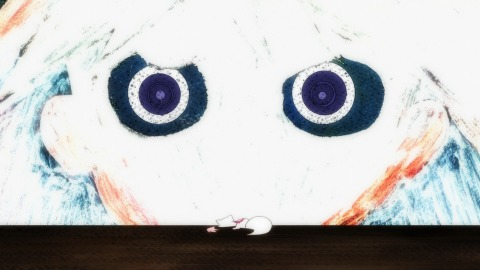
\includegraphics{original.jpg}}
    \caption{Original image}
\end{figure}

\subsection{Full images}

Ordered ascending by the apparent blur radius:

\begin{figure}[H]
    \centering \resizebox*{7cm}{3.9375cm}{
\includegraphics{ifq4.png}}
    \caption{Iterative (modified initial kernel), 4 passes, full image}
\end{figure}

\begin{figure}[H]
    \centering \resizebox*{7cm}{3.9375cm}{
\includegraphics{gf31.png}}
    \caption{Gauss, $r = 31$, full image}
\end{figure}

\begin{figure}[H]
    \centering \resizebox*{7cm}{3.9375cm}{
\includegraphics{if5.png}}
    \caption{Iterative, 5 passes, full image}
\end{figure}

\begin{figure}[H]
    \centering \resizebox*{7cm}{3.9375cm}{
\includegraphics{gf50.jpg}}
    \caption{Gauss, $r = 50$, full image}
\end{figure}

\begin{figure}[H]
    \centering \resizebox*{7cm}{3.9375cm}{
\includegraphics{ifq5.png}}
    \caption{Modified iterative, 5 passes, full image}
\end{figure}

As you can see, the only visible difference is the apparent blur radius. Apart from that, there is no visible quality difference.

\subsection{Downscaled images}

\begin{figure}[H]
    \centering \resizebox*{7cm}{3.9375cm}{
\includegraphics{g2r31.png}}
    \caption{Gauss, $r = 7$, $\frac 1{16}$ image area}
\end{figure}

\begin{figure}[H]
    \centering \resizebox*{7cm}{3.9375cm}{
\includegraphics{g4r31.png}}
    \caption{Gauss, $r = 3$, $\frac 1{64}$ image area}
\end{figure}

The first image still looks good; the second one shows clear artifacts probably due to the small kernel size (a 1080p image still looks fine when blurred at $\frac 1{256}$ of the original size
with $r = 7$).

\subsection{Downscaled movement}

The following images are the amplified (both amplified equally) difference of the image simply blurred and the image moved down by two pixels, then blurred and then moved up again. They reveal the
problem of movement flickering.

\begin{figure}[H]
    \centering \resizebox*{7cm}{3.9375cm}{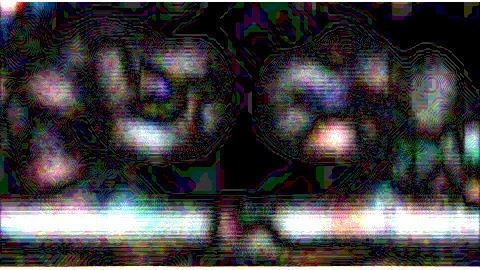
\includegraphics{downscale-diff.jpg}}
    \caption{Movement difference for an image which was downscaled before blurring ($\frac 1{16}$)}
\end{figure}

\begin{figure}[H]
    \centering \resizebox*{7cm}{3.9375cm}{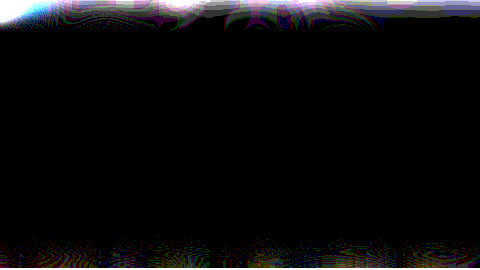
\includegraphics{full-diff.jpg}}
    \caption{Movement difference for an image blurred with the original size}
\end{figure}

The second image exhibits some artifacts due to “foreign” pixels added at the top for moving it down. Other than that, only the bottom has some minor disturbances. The first image however has
clear artifacts all over the image, especially along the borders of the original image.


\newpage

\section{Performance comparison}

Gaussians were performed without built-in bilinear interpolation; however, take into consideration that the apparent blur radius of the iterative approach (especially the modified one) is larger
than the Gaussian radius, so both errors should equal out.

\subsection{AMD HD 7850 with fglrx}

Full-size:
\begin{itemize}
    \item 1920x1080, Gaussian ($r = 127$): \\
        399 ms $\pm$959 $\upmu$s
    \item 1920x1080, iterative (7 passes): \\
        2.72 ms $\pm$139 $\upmu$s
    \item 1920x1080, modified iterative (7 passes): \\
        2.88 ms $\pm$130 $\upmu$s
\end{itemize}

(I cannot explain the extreme value for the Gaussian blur; but it is reproducable, so I am willing to blame the driver)

Downscaled to $\frac 1{16}$:
\begin{itemize}
    \item 480x270, Gaussian ($r = 31$): \\
        893 $\upmu$s $\pm$108 $\upmu$s
    \item 480x270, iterative (5 passes): \\
        656 $\upmu$s $\pm$137 $\upmu$s
    \item 480x270, modified iterative (5 passes): \\
        712 $\upmu$s $\pm$134 $\upmu$s
\end{itemize}

Downscaled to $\frac 1{64}$:
\begin{itemize}
    \item 240x135, Gaussian ($r = 15$): \\
        352 $\upmu$s $\pm$86.5 $\upmu$s
    \item 240x135, iterative (4 passes): \\
        479 $\upmu$s $\pm$79.3 $\upmu$s
    \item 240x135, modified iterative (4 passes): \\
        499 $\upmu$s $\pm$67.9 $\upmu$s
\end{itemize}

Downscaled to $\frac 1{256}$:
\begin{itemize}
    \item 120x67, Gaussian ($r = 7$): \\
        221 $\upmu$s $\pm$82.4 $\upmu$s
    \item 120x67, iterative (3 passes): \\
        378 $\upmu$s $\pm$86.8 $\upmu$s
    \item 120x67, modified iterative (3 passes): \\
        383 $\upmu$s $\pm$81.9 $\upmu$s
\end{itemize}

\newpage

\subsection{AMD HD 7850 with radeon}

Full-size:
\begin{itemize}
    \item 1920x1080, Gaussian ($r = 127$): \\
        n/a (\url{https://bugs.freedesktop.org/show\_bug.cgi?id=75276})
    \item 1920x1080, iterative (7 passes): \\
        3.47 ms $\pm$149 $\upmu$s
    \item 1920x1080, modified iterative (7 passes): \\
        3.72 ms $\pm$160 $\upmu$s
\end{itemize}

Downscaled to $\frac 1{16}$:
\begin{itemize}
    \item 480x270, Gaussian ($r = 31$): \\
        n/a
    \item 480x270, iterative (5 passes): \\
        859 $\upmu$s $\pm$59.3 $\upmu$s
    \item 480x270, modified iterative (5 passes): \\
        990 $\upmu$s $\pm$103 $\upmu$s
\end{itemize}

Downscaled to $\frac 1{64}$:
\begin{itemize}
    \item 240x135, Gaussian ($r = 15$): \\
        701 $\upmu$s $\pm$57.2 $\upmu$s
    \item 240x135, iterative (4 passes): \\
        630 $\upmu$s $\pm$61.2 $\upmu$s
    \item 240x135, modified iterative (4 passes): \\
        702 $\upmu$s $\pm$61.7 $\upmu$s
\end{itemize}

Downscaled to $\frac 1{256}$:
\begin{itemize}
    \item 120x67, Gaussian ($r = 7$): \\
        432 $\upmu$s $\pm$53.9 $\upmu$s
    \item 120x67, iterative (3 passes): \\
        540 $\upmu$s $\pm$49.7 $\upmu$s
    \item 120x67, modified iterative (3 passes): \\
        545 $\upmu$s $\pm$51.2 $\upmu$s
\end{itemize}

\newpage

\subsection{Intel HD 4000}

Full-size:
\begin{itemize}
    \item 1920x1080, Gaussian ($r = 127$): \\
        112 ms $\pm$50.2 ms
    \item 1920x1080, iterative (7 passes): \\
        30.8 $\pm$5.39 ms
    \item 1920x1080, modified iterative (7 passes): \\
        30.7 ms $\pm$5.39 ms
\end{itemize}

Downscaled to $\frac 1{16}$:
\begin{itemize}
    \item 480x270, Gaussian ($r = 31$): \\
        5.42 ms $\pm$90.5 $\upmu$s
    \item 480x270, iterative (5 passes): \\
        2.64 ms $\pm$1.11 ms
    \item 480x270, modified iterative (5 passes): \\
        2.77 ms $\pm$1.17 ms
\end{itemize}

Downscaled to $\frac 1{64}$:
\begin{itemize}
    \item 240x135, Gaussian ($r = 15$): \\
        1.44 ms $\pm$140 $\upmu$s
    \item 240x135, iterative (4 passes): \\
        1.13 ms $\pm$417 $\upmu$s
    \item 240x135, modified iterative (4 passes): \\
        1.17 ms $\pm$348 $\upmu$s
\end{itemize}

Downscaled to $\frac 1{256}$:
\begin{itemize}
    \item 120x67, Gaussian ($r = 7$): \\
        882 $\upmu$s $\pm$367 $\upmu$s
    \item 120x67, iterative (3 passes): \\
        791 $\upmu$s $\pm$429 $\upmu$s
    \item 120x67, modified iterative (3 passes): \\
        814 $\upmu$s $\pm$422 $\upmu$s
\end{itemize}

\newpage

\subsection{Conclusion}

As one can see, the algorithm presented here is useful only for large blur radii ($r > 25$). For smaller radii (which are especially common on small-sized or downscaled textures), the overhead is too
large and the well-known standard algorithm is simply fast enough.

On the other hand, for integrated GPUs without dedicated memory for which texture reads are especially costly, the iterative algorithm is faster even for small blur radii.

\end{document}
